\subsection{Vereinzelung}
sdffd
\newline
\newline
\textbf{Aufbau}
\newline


	\begin{figure}[H]
	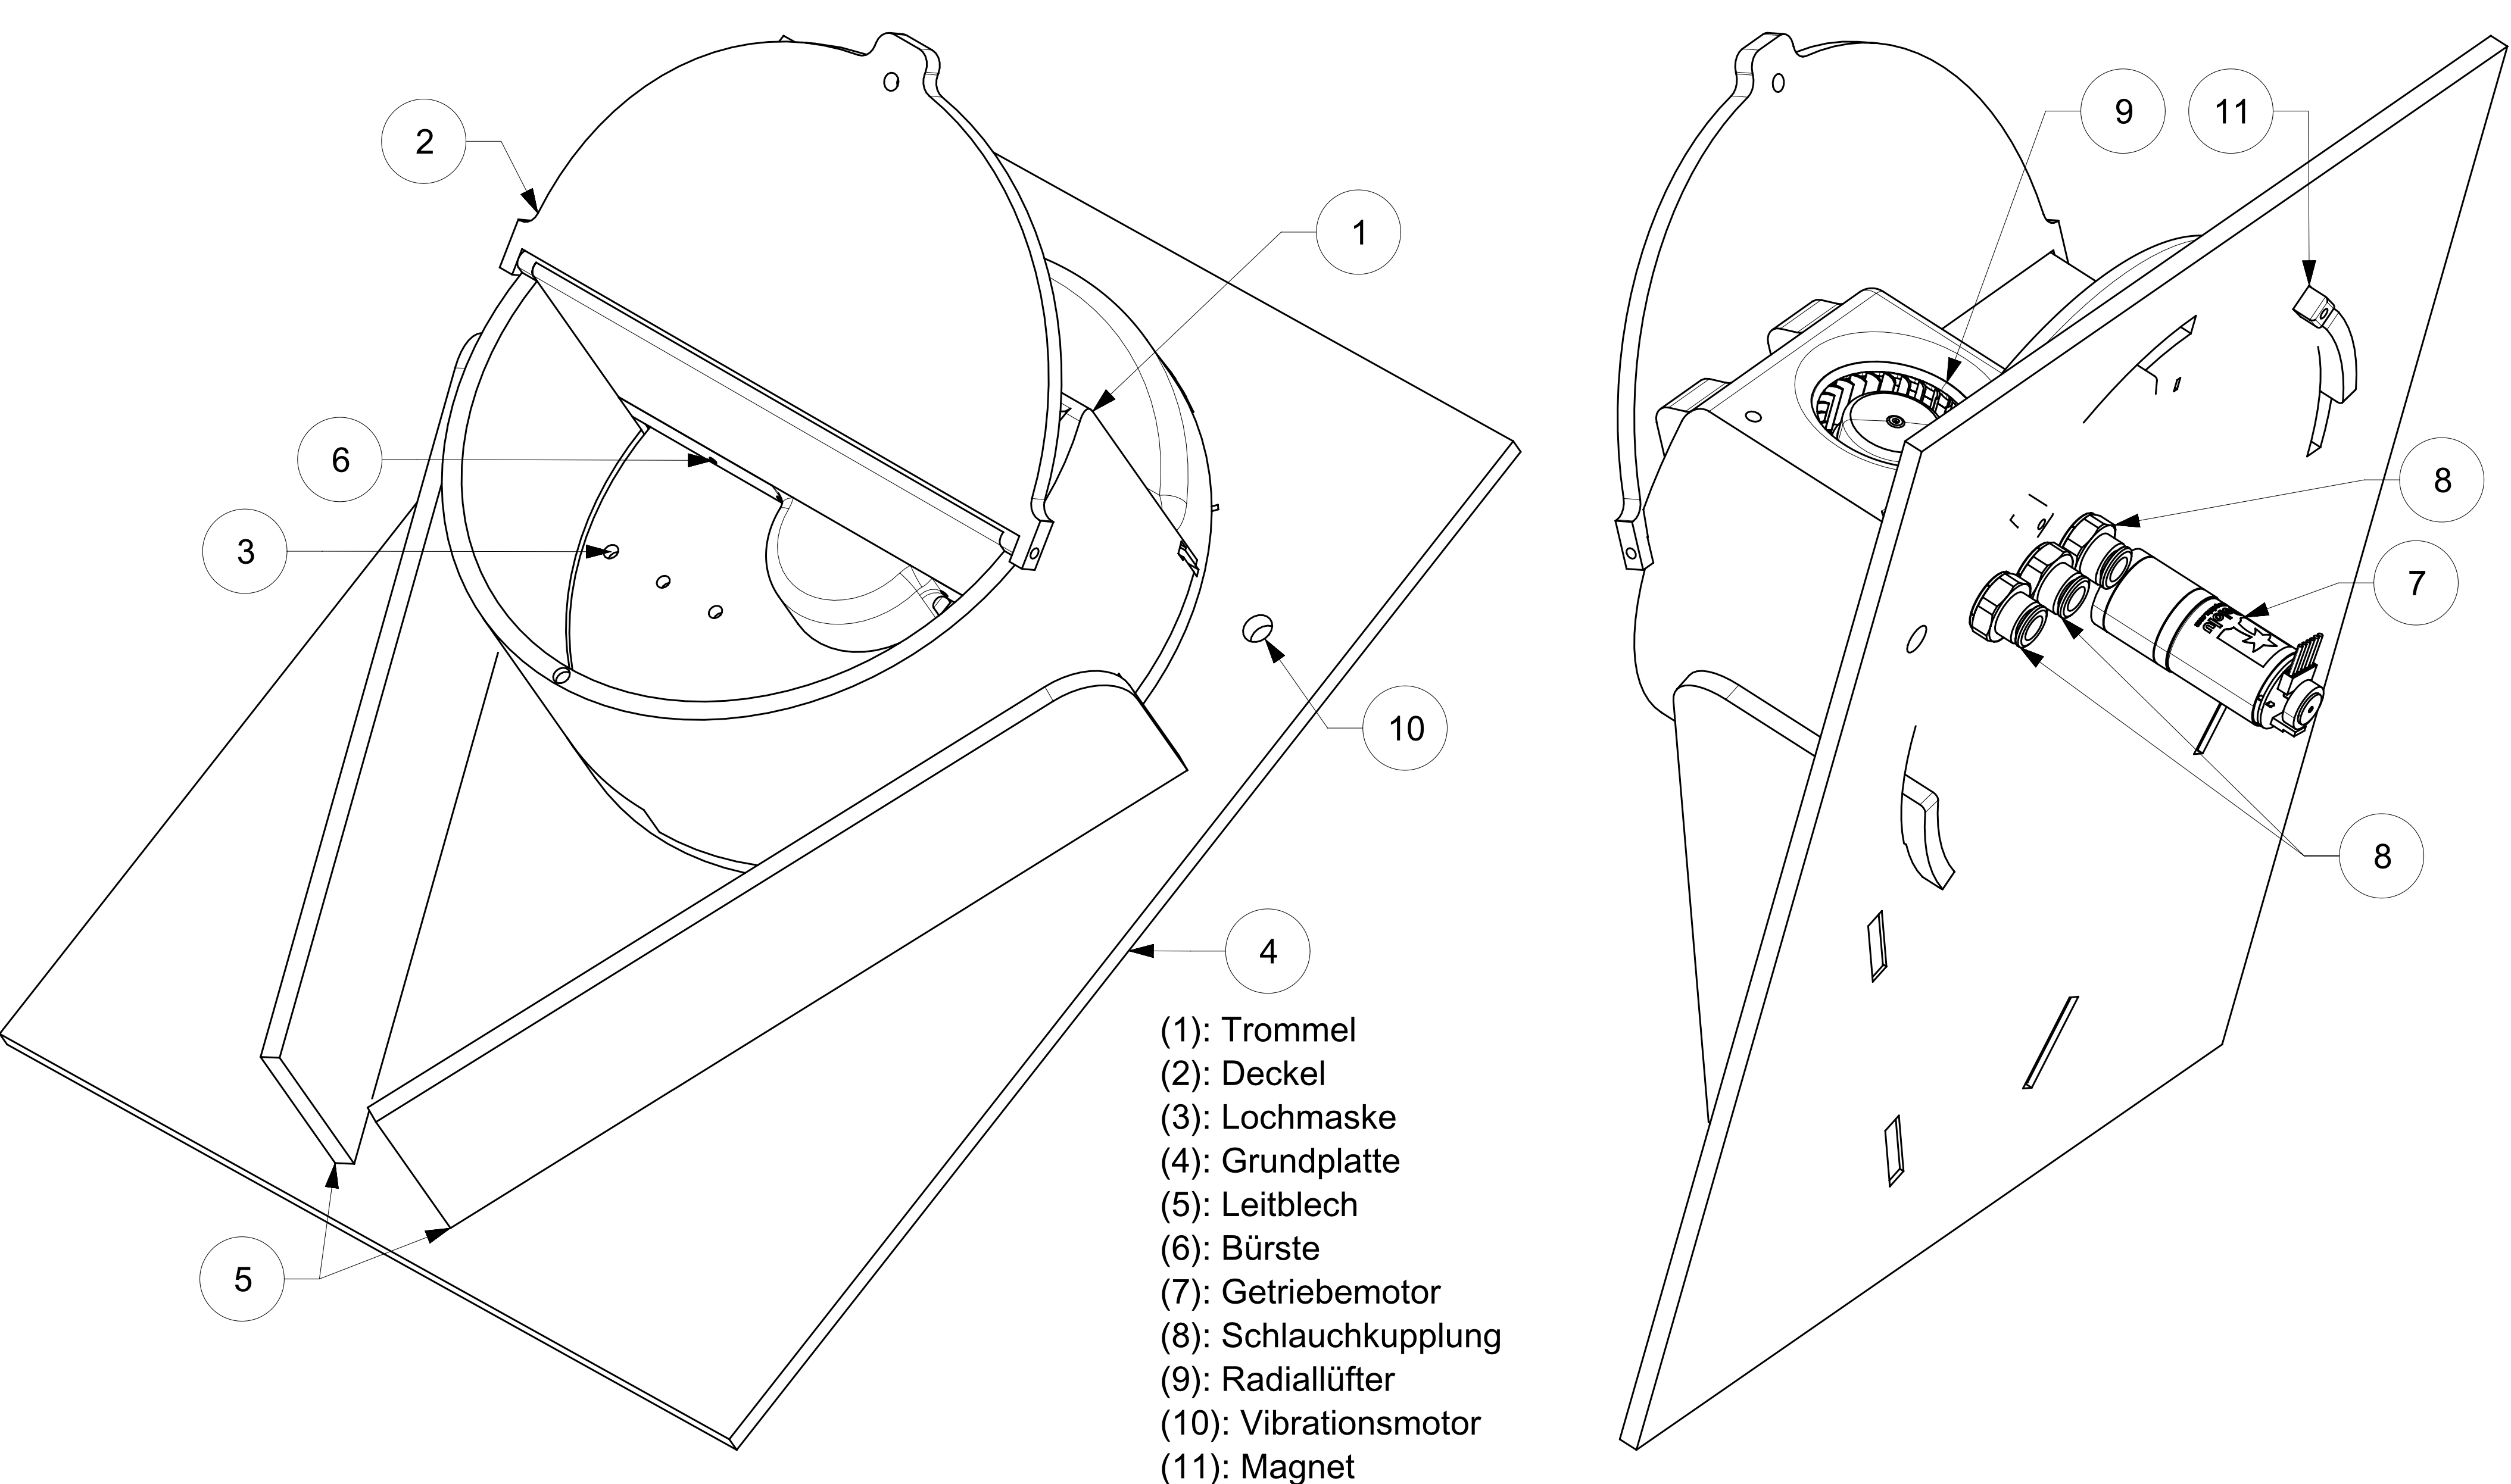
\includegraphics[scale=0.45]{Illustrationen/6-Umsetzung/details_vereinzelung.jpg}
	\caption{Detaillierte Übersicht der Vereinzelung}
	\label{fig:details_vereinzelung}
	\end{figure}
asfasdf
\newline
\textbf{Funktion}
\newline
dfgsdf
\newline
\textbf{Abhilfemassnahmen}
\newline
sadfsdaf
\newline
\textbf{Entleeren}
\newline
	\begin{figure}[H]
	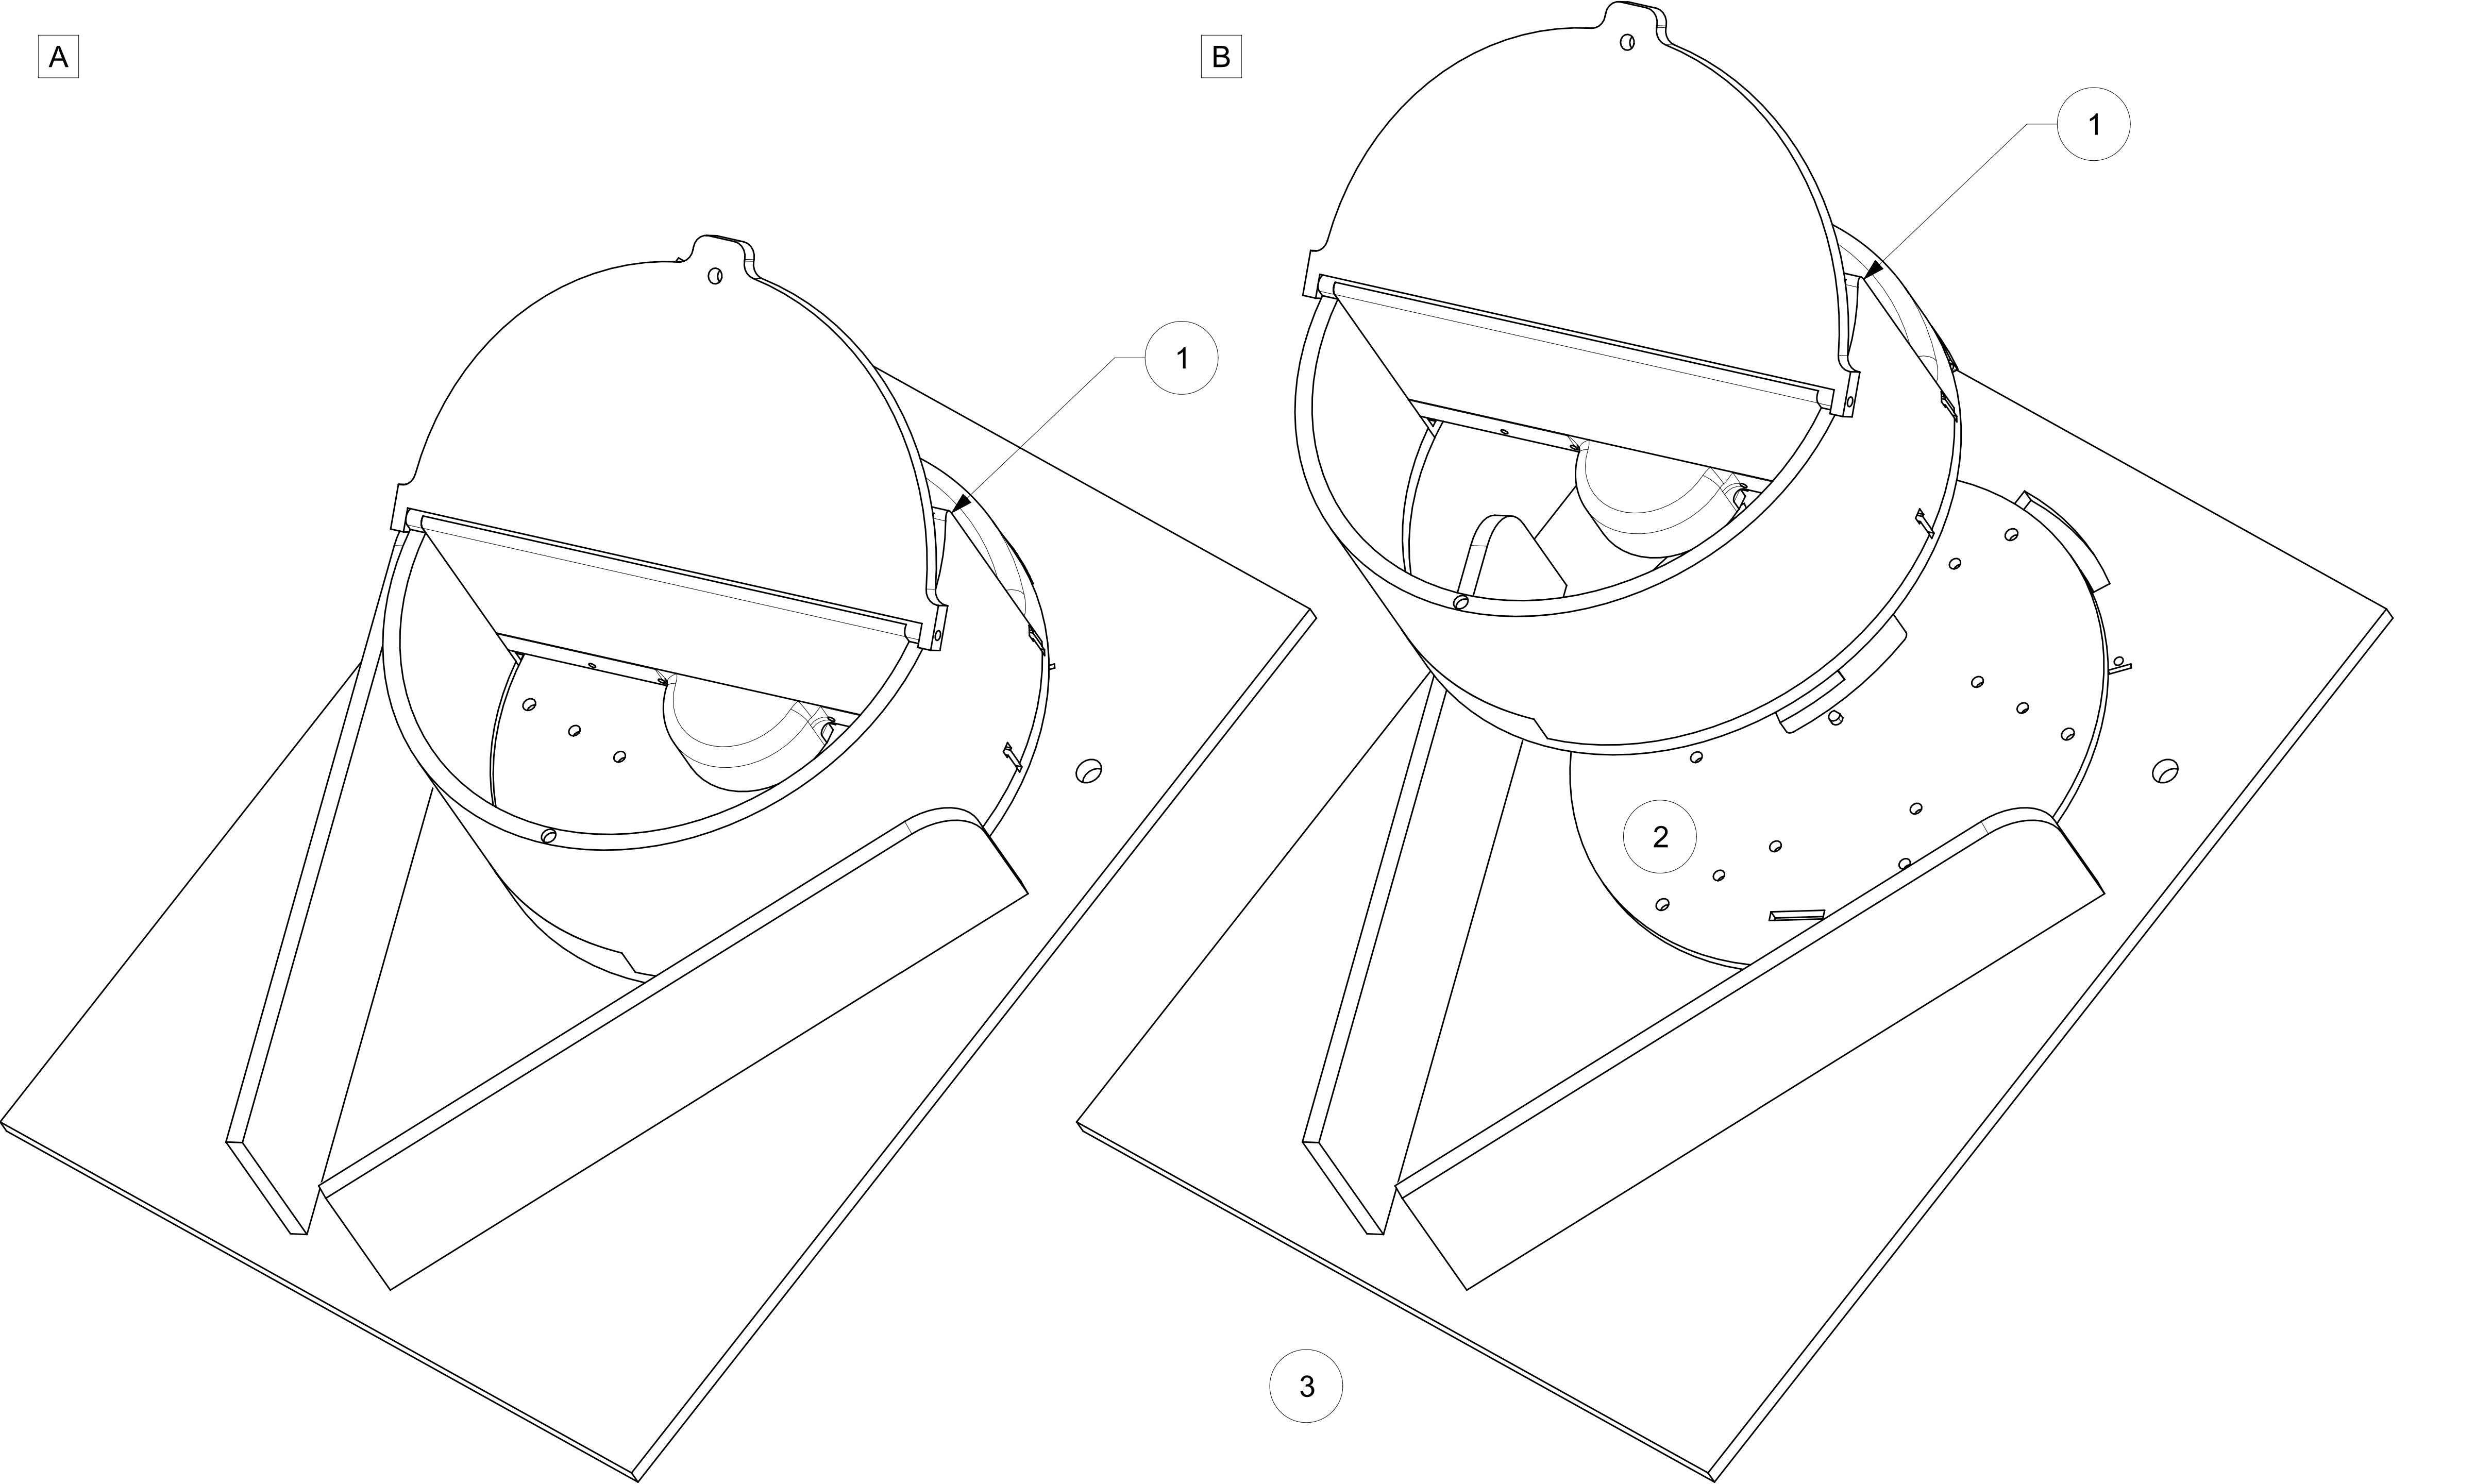
\includegraphics[scale=0.42]{Illustrationen/6-Umsetzung/vereinzelung_entleeren.jpg}
	\caption{Entleerung der Trommel}
	\label{fig:details_vereinzelung}
	\end{figure}
asdfasdf
\newline
\textbf{Lochmaske}
\newline
Detektion
	\begin{figure}[H]
	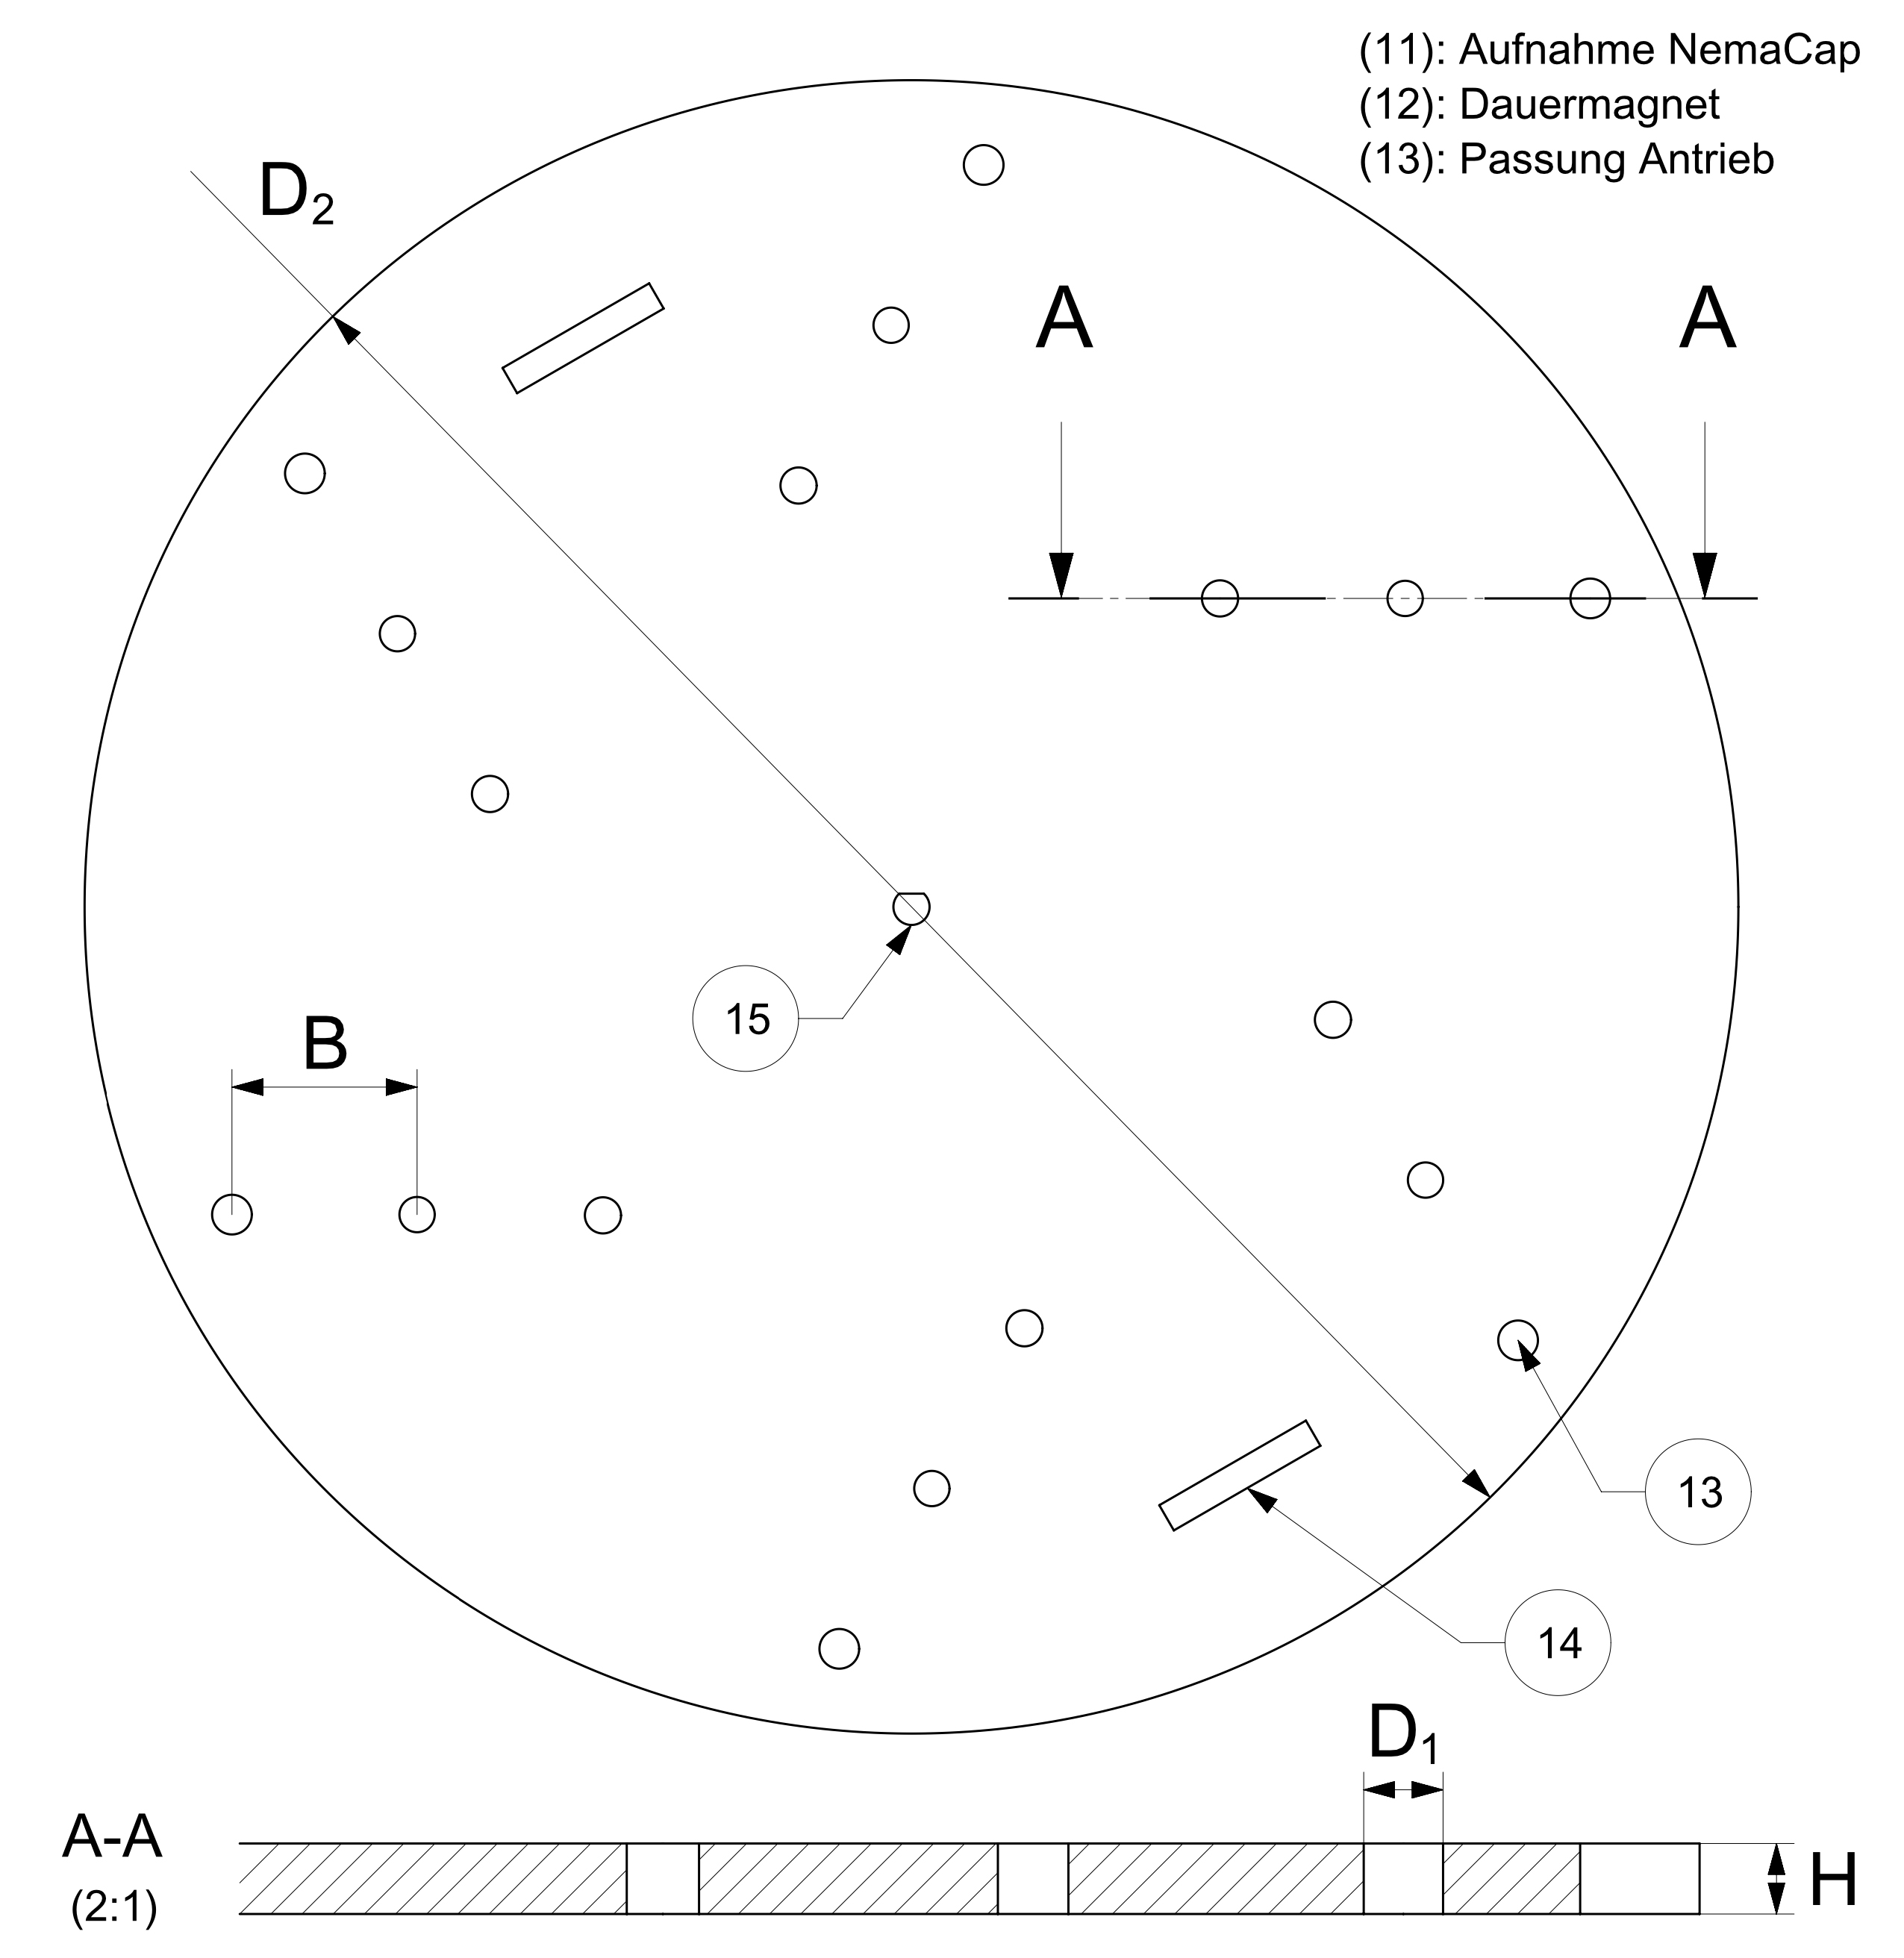
\includegraphics[scale=0.63]{Illustrationen/6-Umsetzung/detail_lochmaske.jpg}
	\caption{Entleerung der Trommel}
	\label{fig:detail_lochmaske}
	\end{figure}
jhj
\newline
\textbf{Fertigungsverfahren und Materialwahl}
\newline